\documentclass{beamer}
\usepackage{ngerman}
\usepackage[utf8]{inputenc}
\usepackage{pgf}
\usepackage{verbatim}
\usepackage{listings}
\usepackage[]{hyperref} 
\usepackage{multicol}
\beamertemplatenavigationsymbolsempty

\usetheme{Szeged}

\title{HadoopDB\\ ein großer Schritt in die falsche Richtung}
\subtitle[]{Seminar 01912\\ Sommersemester 2011}
\date{\today}
\author[T. Koch]{Thomas Koch}
\institute[Fernuni Hagen]{Lehrgebiet Datenbanksysteme für neue Anwendungen\\ Fernuniversität Hagen}

\begin{document}
  \begin{frame}
    \titlepage
  \end{frame}

  \begin{frame}
    \tableofcontents{}
  \end{frame}

\section{Ende einer Ära}
\begin{frame}{Zeiten ändern sich \ldots}
  \begin{itemize}
    \item Hardware: Speicher, Geschwindigkeit
    \item Kosten Mensch/Maschine
    \item Parallelität
    \item Anwendungsbereiche
  \end{itemize}
  aus: The End of an Architectural Era (It’s Time for a Complete Rewrite) von 
Stonebraker, Michael; Abadi, Daniel J. et al.
\end{frame}

\begin{frame}{MapReduce gegen parallele Datenbanken}
  MapReduce: A major step backwards (Stonebraker)
  \begin{itemize}
    \item MapReduce ist nicht neu (und nicht gleich Hadoop)
    \item keine Schemas
    \item keine höhere Abfragesprache
    \item fehlende Features: Import, sekundäre Indizes, Updates, Transaktionen, Integrität, Views
  \end{itemize}
\end{frame}

\section{Benchmarks}
\begin{frame}{}
  maximal 100 Server
  \begin{quote}
     ``Since few data sets in the world even approach a petabyte in size, it is not at all clear how many MR users really need 1.000 nodes.'' (Stonebraker)
  \end{quote}
  \begin{quote}<2>
     ``I think there is a world market for maybe five computers''
   
     ``640K ought to be enough for anybody''
  \end{quote}
\end{frame}

\begin{frame}{Kritik der Benchmarks}
  \begin{itemize}
    \item keine (echte) Fehlertoleranz
    \item Datenladephase
    \item Problemarten
  \end{itemize}
\end{frame}

\section{HadoopDB}

\begin{frame}{Anforderungen}
  \begin{itemize}
    \item Performanz
    \item Fehlertoleranz
    \item Heterogene Server
    \item Flexible / Erweiterbare Abfrageschnittstelle
  \end{itemize}
  (Energieeffizienz?)
\end{frame}

\begin{frame}{Architektur}
  \begin{center}
    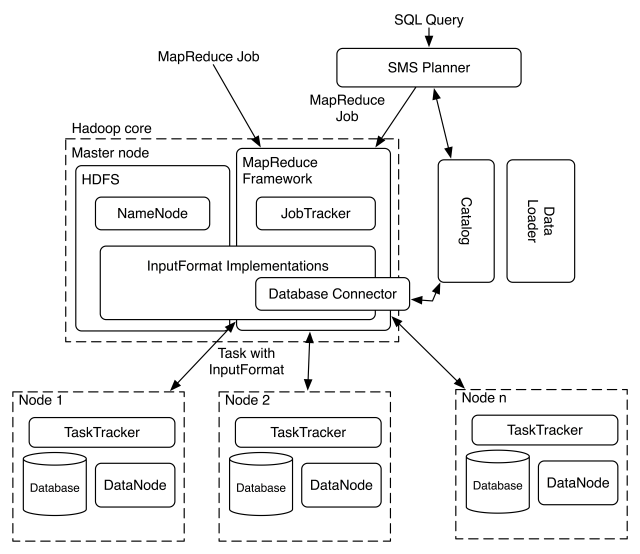
\includegraphics[width=0.7\textwidth]{../ausarbeitung/images/hadoopdb-arch.png}    
  \end{center}
\end{frame}

\begin{frame}{Datenladephase}
  \begin{enumerate}
    \item globaler Hasher (2r, 2w + 1 network copy)
    \item Export ins lokale Dateisystem (1r, 1w)
    \item lokaler Hasher (1r, 1w)
    \item Import in lokale Datenbank (1r, 1w + Indizes)
  \end{enumerate}
\end{frame}

\subsection{Benchmarks}
\subsection{Praktische Evaluation}
\section{Hive}

\end{document}